%!TEX root = hw1.tex
\problem{1}
\paragraph{a)} 
For the $O(n^2)$ solution we compute the intersection between one segment and the rest of the segments. Then we remove that segment and recursively compute the intersections between the rest of the segments.

\begin{algorithm}
	\caption{$O(n^2)$ solution}
	\begin{algorithmic}
	  \Function{intersections}{$P[1..n]$ , $Q[1..n]$}
	  	\State $i \gets $ \Call{findIntersectionsWithSegment}{$P[1]$, $Q[1..n]$} \Comment{O(n)}
		\State \Call{removePointAt}{{$i+1$, $Q[1..n]$}} \Comment{O(n)}
	
		\Return $i + \Call{intersections}{$P[2..n]$, $Q[1..n-1]$}$
	  \EndFunction
	
	  \Function{findIntersectionsWithSegment}{$p$ , $Q[1..n]$}
		\State $i \gets 0$
		\While{$Q[i] < p$}
			\State $i \gets i + 1$
		\EndWhile
	
		\Return $i$
	  \EndFunction
	
	  \Function{removePoint}{$i$, $Q[1..n]$}
		\For{$j \gets i, n-1$}
			\State $Q[i] \gets Q[i + 1]$
		\EndFor
	  \EndFunction
	\end{algorithmic}
\end{algorithm}

\paragraph{Runtime analysis}
Functions $findIntersectionWithSegment$ and $removePoint$ have a runtime of $O(n)$ since in the worst case scenario they traverse over all all the points. The runtime of $intersections$ is analyzed below:

\clearpage
$I(n) =$ worst case runtime of function $intersections$

$I(n) = I(n - 1) + 2 * O(n)$

\begin{figure}[H]
    \centering
    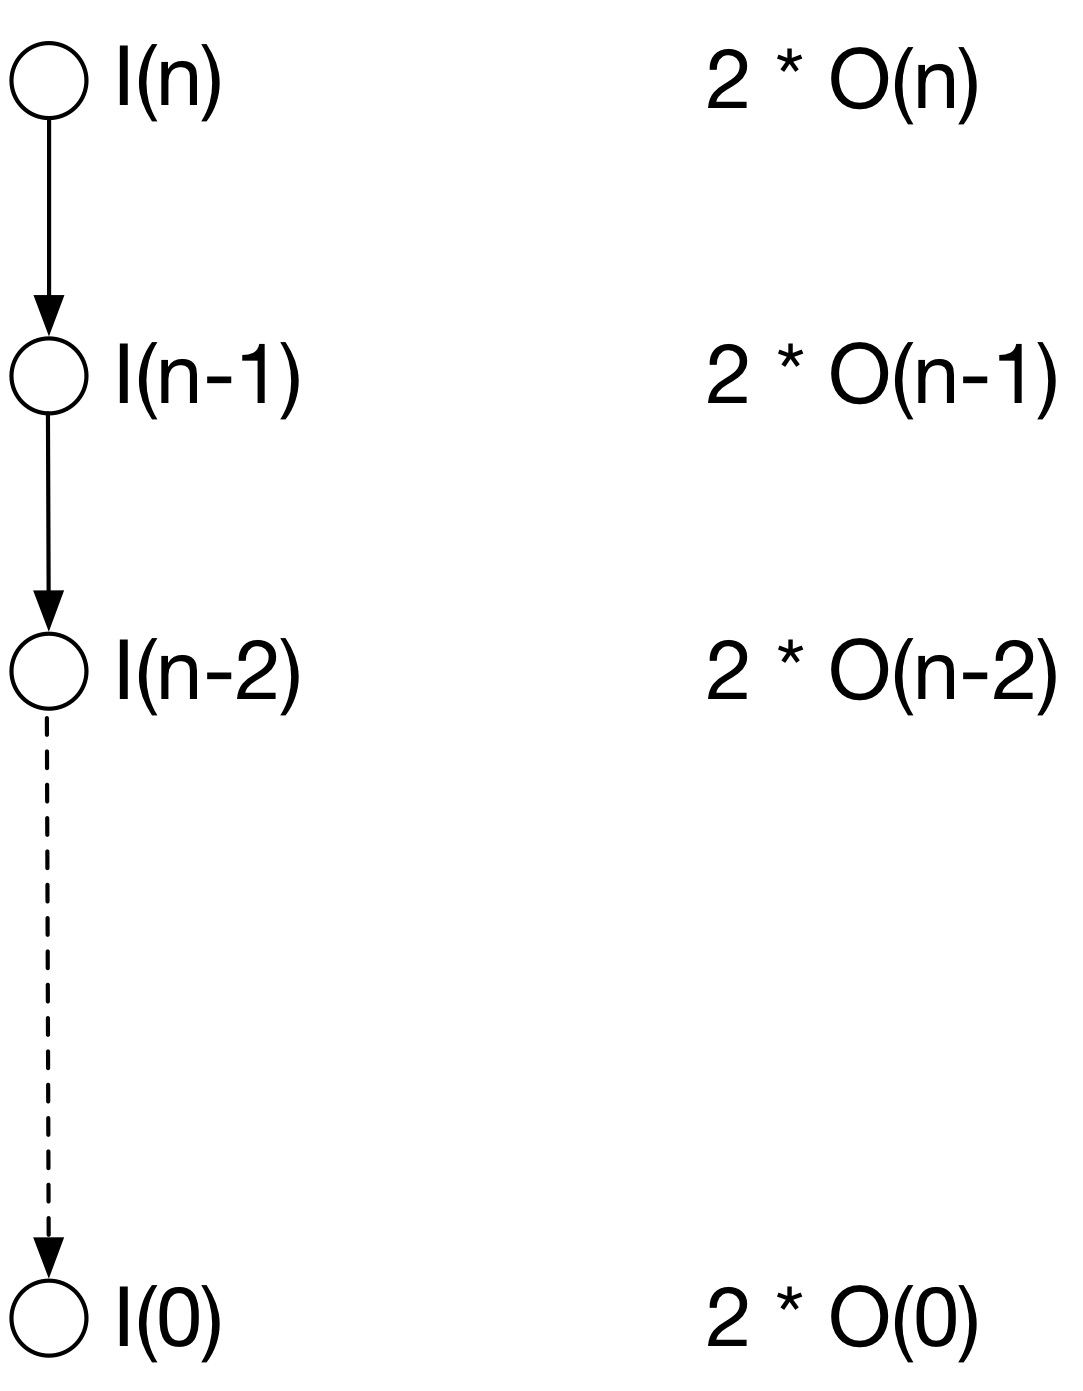
\includegraphics[scale=0.5]{1a)}
\end{figure}

$I(n) = \sum_{i=0}^{n} 2 * O(i) = 2 * \sum_{i=0}^{n} O(i) \Rightarrow  2 * O(n^2) \Rightarrow  O(2 * n^2) \Rightarrow O(n^2)$

